\documentclass{article}
\usepackage[utf8]{inputenc}

\usepackage[T1]{fontenc}
\usepackage{amssymb}
\usepackage[swedish]{babel}
\usepackage{amsmath}
\usepackage{lmodern}
\usepackage{units}
\usepackage{icomma}
\usepackage{color}
\usepackage{graphicx}
\usepackage{bbm}
\usepackage{hyperref}
\usepackage{pdfpages}
\usepackage[makeroom]{cancel}

\setlength{\parindent}{0em}
\setlength{\parskip}{0.5em}

\begin{document}

\begin{titlepage} \newcommand{\HRule}{\rule{\linewidth}{0.3mm}}
\center
\textsc{\Large Chalmers tekniska högskola}\\[0.05cm] % Name of your university/college \textsc{\normalsize Teknisk Matematik}\\[0.2cm]
%\normalsize \\ % Major heading such as course name
\normalsize \today

\HRule \\[0.08cm]
{ \large Planeringsrapport \\ \normalsize{-- Programmering som undervisningsverktyg för signalteori}}\\[0.08cm]
\HRule \\[0.3cm]

\begin{minipage}{0.5\textwidth}
\begin{flushleft} \small
\emph{Författare: Jacob Jonsson, Filip Lindahl, Peter Ngo, Joakim Olsson, Cecilia Rosvall}
\end{flushleft}

\end{minipage}


\end{titlepage}
%\newpage
%\tableofcontents
%\newpage


\section{Bakgrund}
Det har funnits en lång trend på utbildningen för Datateknik på
Chalmers där studenterna haft svårigheter med kurserna “Transformer,
Signaler och System” (TSS) och “Reglerteknik”
%PaJa: "eftersom" verkar vara spekulation
eftersom de bygger på kunskap inom matematik, ett ämne som studenterna
inte fått arbeta med på ungefär ett år.
%
Dessa svårigheter syns bland annat i statistiken för hur många som
klarar kurserna, under perioden från 2010 till 2016 blev i genomsnitt
49\% av alla som skrev tentamen underkända i TSS och under samma
period blev 47\% underkända i Reglerteknik.

%PaJa: "för att stävja denna trend" är en för negativ formulering: se http://wiki.portal.chalmers.se/cse/pmwiki.php/FP/DSLsofMath: "For example, for CS and CSE students we will measure the percentage of students who, having taken DSLM, pass the third-year courses Transforms, signals and systems and Control Theory (Reglerteknik), which are current major stumbling blocks."
För att minska svårigheterna som studenterna har för dessa kurser
påbörjades ett pedagogiskt projekt (DSLsOfMath) som hittills
resulterat i kursen “Matematikens domänspecifika språk”, där man
använder funktionell programmering som är ett verktyg som
studenterna har erfarenhet av och som använder en notation med
fokus på tydlighet för att lära ut matematiska begrepp.

Vårt projekt uppstod som en avgrening av DSLsOfMath-projektet och
fokuserar mer på signal- och systemteoretiska färdigheter snarare än
en allmän matematisk grund.

\section{Syfte}
Syftet med projektet är att underlätta för studenter inom datateknik
att ta till sig signal- och systemteoretiska ämnen genom att utnyttja
deras kunskaper inom programmering och även göra det möjligt att
betrakta ämnet ur en programmerares perspektiv.
%
Vi vill göra gapet mellan datateknik och signalteori mindre för att
minska problemen som nämns i bakgrundsavsnittet.

Projektet är tänkt att resultera i en handledningsguide, en så kallad
tutorial, som kan fungera som ett komplement till de kurser som ges
inom signalteori på den datatekniska grundutbildningen.
%
Denna guide ska innehålla förklaringar och programmeringsövningar som
är anpassade för studenter på den datatekniska utbildningen.

\section{Programanalys}
Uppgiften i detta projekt kommer bestå i att utarbeta en produkt som
komplement till kurserna “Reglerteknik” och “Transformer, signaler och
system”.
%PaJa: "produkt" låter lite styltigt och allmänt. Kanske "lärmaterial"?
%
För att kunna utveckla denna produkt kommer först omfattande
förstudier behöva bedrivas innan vi utvecklar vår produkt och denna
produkt kommer sedan behöva testas.

\subsection{Förstudier}
För att få reda på var de största svårigheterna med förståelsen inom
ämnena och vad som kan göras för att lätta på dessa problem behöver vi
först undersöka var dessa svårigheter ligger.
%
Detta kan göras genom att intervjua studenterna som har gått kursena
samt examinatorerna och lärarna för kurserna.

För att kunna skriva en produkt med bra innehåll kommer vi även behöva
bedriva en hel del efterforskningar och litteraturstudier inom såväl
pedagogik som de signalteoretiska ämnen vi beskriver.

\subsection{Produkten}
Efter förstudierna kommer produkten utvecklas.
%
Denna kommer bestå av både löpande text och programmeringskod.
%
Innehållet kommer bestå av förklarande teori, exempeluppgifter samt
övningsuppgifter med tillhörande lösningar.

\subsection{Testa produkten}
Produkten kommer sedan behöva testas på den aktuella målgruppen för
möjligheten att uppdatera och förbättra den slutgiltiga produkten.

\section{Avgränsning}
I denna projekt skrivs en handlednings guide vars avsikt är att
förtydliga de delar studenter inom datateknik finner svårt i kurserna
“Transform, Signal och System” och “Reglerteknik”.
%
Detta innebär att vi endast fokuserar på svårigheter inom dessa kurser
och inte en handlednings guide som täcker hela själva ämnet.
%
Det vill säga, produkten kommer inte bli ett underlag för motsvarande
kurs DAT325 utan en komplement till kurserna SSY080 och ERE102.

\section{Metod}
\subsection{Förstudier}
För att samla in information om vilka moment i kurserna TSS och
Reglerteknik som datastudenter har svårast för planerar vi att
intervjua examinatorerna inom båda kurserna.

Vi kommer också fråga studenter som läst kurserna vad de tyckte var
svårast.

\subsection{Produkten}
För att kunna skapa produkten som syftar på att lära studenter om
signalteoretiska begrepp på ett lättillgängligt sätt kommer vi studera
pedagogik och alternativa inlärningsformer som exempelvis boken och
hemsidan “Learn you a Haskell for great good”.

Rent strukturellt planerar vi att dela upp momenten i sex delavsnitt
som kommer att innehålla runt 15 - 20 uppgifter vardera där
studenterna får lära sig om signalteori genom att implementera de
inblandade typerna och relationerna som domänspecifika språk i
Haskell.

\subsection{Testa Produkten}
För att testa svårighetsgraden på vår produkt kommer vi dels att testa
gruppens uppgifter internt och förhoppningsvis hitta utomstående
studenter som är villiga att testa det åt oss.
%
Vi kommer ge feedback internt på uppgifterna och även förhoppningsvis
få feedback från de utomstående som testar produkten så vi kan
vidareutveckla produkten.

\section{Tidsplan}
\subsection{Milstolpar och delmål}
\begin{itemize}
\item 10:e feb - Planeringsrapport och grov planering klar
\item 11:e feb - Fackspråkshandledningstillfälle 1
\item 12:e feb - Planeringsrapport inlämning
\item 24:e feb - Intervjuer, grundläggande efterforskningar om tss och reglerkurserna klara
\item 24:e feb - Litteraturstudier inom pedagogik klara
\item 1:e mars - Utkast för grov tutorial klar (uppgifter ej klara)
\item 1:a mars - Få klart ett litet avsnitt för halvtidsredovisningen, med förslag på uppgifter och text
\item 1:a mars - Halvtidsredovisning
\item 15:e mars - Uppgifter och utkast till text för två av sex delavsnitt i tutorial klara
\item 22:e mars - Första utkast till rapporten klart
\item 22:e mars - Fackspråkshandledningstillfälle 2
\item 28:e mars - Bearbetning av feedback från fackspråk
\item 28:e mars - Påsk
\item 11:e april - Uppgifter och utkast till text för fyra av sex delavsnitt i tutorial klara
\item 25:e april - Uppgifter och utkast till alla delavsnitt i tutorial klara
\item 27:e april - Eventuell engelsk (forskningsinriktad) uppsats klar
\item 28:e april - Andra utkast till rapporten klart
\item 4:e maj - Tutorial klar och testad
\item 11:e maj - Rapporten klar
\item 13:e maj - Fackspråkshandledningstillfälle 3
\item 16:e maj - Rapportinlämning
\item 17:e maj - Utställning
\item 26:e maj - Deadline för opposition
\item 26:e - 27:e maj - Slutredovisning
\item 1:a juni - Sista inlämningen
\end{itemize}

\newpage
\subsection{Gannt schema}
\begin{figure}
    \centering
    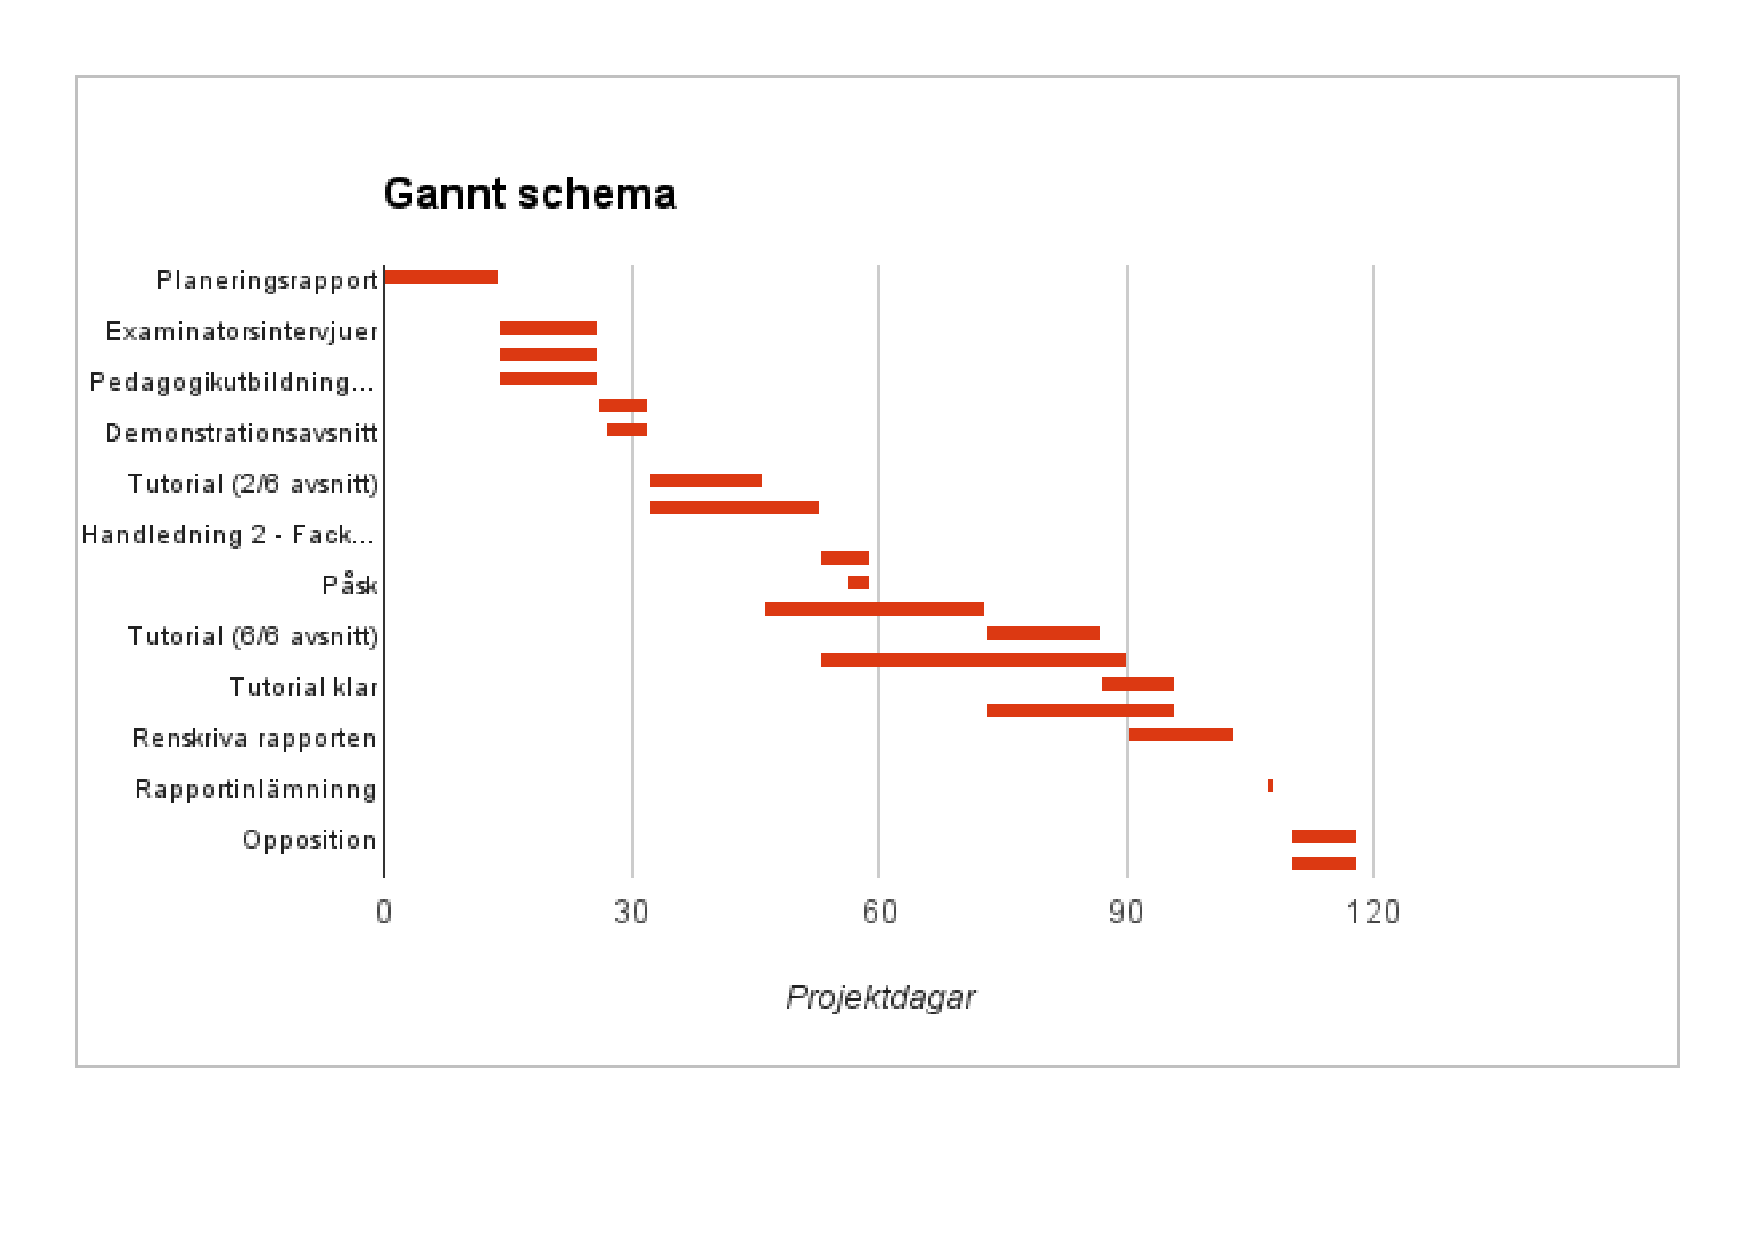
\includepdf[width=0.8\paperwidth]{Gannt}
\end{figure}
\end{document}
